% Lecture notes of AINIT HS26, weekend 2, Friday 08:15 to 12:00: the inner product, the nearest neighbor
% classifier, the matrix product and matrix factorization. The tables come from generated/, written by
% tools/notes_numbers.py, which computes every number from the games' data. Build: see CLAUDE.md.
\documentclass[11pt,a4paper]{article}
\usepackage[margin=2.5cm]{geometry}
\usepackage[T1]{fontenc}
\usepackage{lmodern}
\usepackage{microtype}
\usepackage{amsmath}
\usepackage{array}
\usepackage{tikz}
\usetikzlibrary{matrix,fit}
\usepackage{enumitem}
\usepackage{needspace}
\setlist{nosep, topsep=2pt}
\usepackage[hidelinks]{hyperref}
\urlstyle{same}
\hypersetup{pdftitle={Nearest neighbors, matrix product, matrix factorization},
  pdfauthor={Carlos Cotrini}, pdfsubject={AI in Industry, ETH Zurich, weekend 2, lecture notes}}
\setlength{\parindent}{0pt}
\setlength{\parskip}{5pt plus 1pt}
\renewcommand{\arraystretch}{1.15}

\newcommand{\term}[1]{\textbf{#1}}
\newlength{\headwidth}  % set by the generated figures
\newcommand{\VideoStore}{\href{https://eth-ainit-hs26.github.io/AINIT-PAGE/viz/we2/video-store/}{Once Upon a Video Store}}
\newcommand{\PartOne}{\href{https://eth-ainit-hs26.github.io/AINIT-PAGE/viz/we2/matchmaker-part-1/}{Matchmaker, part one}}
\newcommand{\PartTwo}{\href{https://eth-ainit-hs26.github.io/AINIT-PAGE/viz/we2/matchmaker-part-2/}{Matchmaker, part two}}
\newcommand{\PartThree}{\href{https://eth-ainit-hs26.github.io/AINIT-PAGE/viz/we2/matchmaker-part-3/}{Matchmaker, part three}}
\newcommand{\Optional}{\href{https://eth-ainit-hs26.github.io/AINIT-PAGE/viz/we2/matchmaker-optional/}{Matchmaker, optional part}}
\newcommand{\NotebookNN}{\href{https://colab.research.google.com/github/eth-ainit-hs26/w2-cx-public/blob/main/01_cx_nearest_neighbours_student.ipynb}{nearest neighbors}}
\newcommand{\NotebookMF}{\href{https://colab.research.google.com/github/eth-ainit-hs26/w2-cx-public/blob/main/02_cx_matrix_factorization_student.ipynb}{matrix factorization}}
\newcommand{\NotebookOpt}{\href{https://colab.research.google.com/github/eth-ainit-hs26/w2-cx-public/blob/main/02_cx_matrix_factorization_optional_student.ipynb}{matrix factorization, optional}}

\begin{document}

{\LARGE\bfseries\raggedright Nearest neighbors, matrix product,\\ matrix factorization\par}
\smallskip
Lecture notes. AI in Industry, ETH Zurich, weekend 2, Friday 13 November 2026, 08:15 to 12:00.

\section{The inner product}

\term{Rating.} A number from $-2$ to $2$: $2$ loved, $1$ liked, $0$ neutral, $-1$ disliked, $-2$ hated. A rating
of 1 to 5 stars becomes the number of stars minus 3.

\term{Customer.} A row of ratings, one per film.

\term{Inner product.} Of two rows of the same length, $a = (a_1, \dots, a_n)$ and $b = (b_1, \dots, b_n)$: the sum
of the products of their entries,
\[ a \cdot b = a_1 b_1 + a_2 b_2 + \dots + a_n b_n. \]

\term{One film.} The product of two customers' ratings says how much they agree: positive when both are on the
same side, negative when they are on opposite sides, $0$ when one of them is neutral, further from $0$ when the
opinions are stronger. Jaws: Ivo and Pia, $2 \times 2 = 4$; Ivo and Rosa, $2 \times (-2) = -4$; Pia and Kai,
$2 \times 1 = 2$; Kai and Tom, $1 \times (-1) = -1$.

\term{Several films.} The inner product adds the agreements of all films. Vera and Kai:
\begin{center}
% GENERATED by tools/notes_numbers.py: do not edit, run the script.
\begin{tabular}{l*{7}{c}}
 & Jaws & & The Shining & & Notting Hill \\
Vera & $2$ & & $1$ & & $-1$ \\
Kai & $1$ & & $2$ & & $-2$ \\ \cline{2-6}
 & $2$ & $+$ & $2$ & $+$ & $2$ & $=$ & $6$ \\
\end{tabular}

\end{center}

With ratings $1$ and $-1$ only, the inner product is the number of matches minus the number of mismatches.

Game: \VideoStore, acts 1 to 3.

\section{The nearest neighbor classifier}

\term{Classifier.} A rule that predicts the class of a new case. Here the case is a newcomer, and the class is her
rating of a film she has not seen.

\term{Nearest neighbor classifier.}
\begin{enumerate}
\item Similarity: the inner product of the newcomer's row with each regular customer's row, on the films the
  newcomer rated.
\item Nearest neighbor: the regular with the largest inner product.
\item Prediction: the nearest neighbor's rating of the film.
\end{enumerate}

\term{$k$ nearest neighbors.} The $k$ regulars with the largest inner products vote with their ratings of the film.
The prediction is the rating with the most votes; on a tie, the nearer neighbor's vote wins.

\needspace{12\baselineskip}
Example. Vera rated three films. The regulars, sorted by their inner product with her:
\begin{center}
% GENERATED by tools/notes_numbers.py: do not edit, run the script.
\begin{tabular}{|l|c|c|c|c|c|}
\hline
 & Jaws & The Shining & Notting Hill & Love Actually & \begin{tabular}[b]{@{}c@{}}inner product\\with Vera\end{tabular} \\ \hline
Vera & $2$ & $1$ & $-1$ & ? & \\ \hline\hline
Kai & $1$ & $2$ & $-2$ & $-2$ & $6$ \\ \hline
Pia & $2$ & $1$ & $2$ & $2$ & $3$ \\ \hline
Ivo & $2$ & $-2$ & $0$ & $1$ & $2$ \\ \hline
Jana & $0$ & $1$ & $0$ & $0$ & $1$ \\ \hline
Tom & $-1$ & $-2$ & $-1$ & $-1$ & $-3$ \\ \hline
Rosa & $-2$ & $-1$ & $2$ & $2$ & $-7$ \\ \hline
\end{tabular}

\end{center}
Nearest neighbor: Kai, $6$. Prediction for Love Actually: $-2$, Kai's rating. Vera's rating after watching it: $-2$.

A count of exact matches picks Pia (two films) over Kai (none); Pia's rating of Love Actually is $2$. The inner
product weighs each agreement by the strength of both ratings.

Game: \VideoStore, act 4. Notebook: \NotebookNN.

\section{The matrix product}

\term{Matrix.} A table of numbers. Its size is $n \times m$: $n$ rows, $m$ columns.

\term{Profiles.} Each customer answers three questions with a number from $-2$ to $2$: real story ($2$) or fiction
($-2$), comedy ($2$) or drama ($-2$), action ($2$) or calm ($-2$). A film critic answers the same questions for
every film. $P$ holds the customers' answers, one row per customer. $Q$ holds the critic's answers, one column per
film.

\term{Embedding.} The numbers that describe a customer (a row of $P$) or a film (a column of $Q$).

\term{Score.} The inner product of a customer's row and a film's column. The higher the score, the better the film
suits the customer.

\term{Matrix product.} $P$ of size $n \times k$ times $Q$ of size $k \times m$, defined when $P$ has as many columns
as $Q$ has rows. $PQ$ has size $n \times m$. Its entry in row $i$ and column $j$ is the inner product of row $i$ of
$P$ and column $j$ of $Q$. With $Q$ drawn above $PQ$ and $P$ on its left, each entry sits where its row and its
column meet:
\begin{center}
% GENERATED by tools/notes_numbers.py: do not edit, run the script.
\settowidth{\headwidth}{\footnotesize\begin{tabular}{@{}c@{}}13\\Apollo\\Black\\Interstellar\\Intouchables\\Men\\The\\in\end{tabular}}
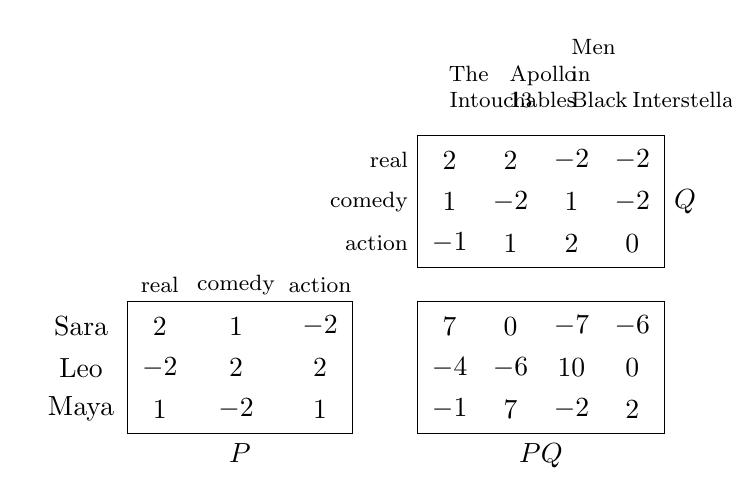
\begin{tikzpicture}
\matrix (m) [matrix of nodes, nodes in empty cells, row sep=1.5pt, column sep=3pt,
  nodes={minimum height=1.35em, minimum width=1.9em, anchor=center, inner sep=1pt}, column 1/.style={anchor=east}] {
 &  &  &  &  & |[text width=\headwidth, align=center, anchor=south, minimum height=0pt, font=\footnotesize]| The Intouchables\strut & |[text width=\headwidth, align=center, anchor=south, minimum height=0pt, font=\footnotesize]| Apollo 13\strut & |[text width=\headwidth, align=center, anchor=south, minimum height=0pt, font=\footnotesize]| Men in Black\strut & |[text width=\headwidth, align=center, anchor=south, minimum height=0pt, font=\footnotesize]| Interstellar\strut \\
 &  &  &  &  & $2$ & $2$ & $-2$ & $-2$ \\
 &  &  &  &  & $1$ & $-2$ & $1$ & $-2$ \\
 &  &  &  &  & $-1$ & $1$ & $2$ & $0$ \\
 & |[font=\footnotesize]| real & |[font=\footnotesize]| comedy & |[font=\footnotesize]| action &  &  &  &  &  \\
|[inner xsep=4pt]| Sara & $2$ & $1$ & $-2$ &  & $7$ & $0$ & $-7$ & $-6$ \\
|[inner xsep=4pt]| Leo & $-2$ & $2$ & $2$ &  & $-4$ & $-6$ & $10$ & $0$ \\
|[inner xsep=4pt]| Maya & $1$ & $-2$ & $1$ &  & $-1$ & $7$ & $-2$ & $2$ \\
};
\node[draw, inner sep=2pt, fit=(m-2-6)(m-4-9)] (Q) {};
\node[draw, inner sep=2pt, fit=(m-6-2)(m-8-4)] (P) {};
\node[draw, inner sep=2pt, fit=(m-6-6)(m-8-9)] (PQ) {};
\node[anchor=east, inner sep=3pt, font=\footnotesize] at (Q.west |- m-2-6) {real};
\node[anchor=east, inner sep=3pt, font=\footnotesize] at (Q.west |- m-3-6) {comedy};
\node[anchor=east, inner sep=3pt, font=\footnotesize] at (Q.west |- m-4-6) {action};
\node[anchor=west, inner sep=3pt] at (Q.east) {$Q$};
\node[anchor=north, inner sep=3pt] at (P.south) {$P$};
\node[anchor=north, inner sep=3pt] at (PQ.south) {$PQ$};
\end{tikzpicture}

\end{center}
Sara and The Intouchables: $2 \times 2 + 1 \times 1 + (-2) \times (-1) = 4 + 1 + 2 = 7$. Each customer's highest
score: Sara, The Intouchables ($7$); Leo, Men in Black ($10$); Maya, Apollo 13 ($7$).

Sizes: $5 \times 4$ times $4 \times 6$ gives $5 \times 6$. The product of $2 \times 3$ and $4 \times 2$ is
undefined: $3$ columns against $4$ rows.

Game: \PartOne. Notebook: \NotebookMF, part 1.

\section{Matrix factorization}

\subsection{The problem}

\term{Matrix factorization.} Given only the ratings $R$, $n$ customers by $m$ films, find $P$ ($n \times k$) and
$Q$ ($k \times m$) whose product $PQ$ is close to $R$. The number $k$ is chosen in advance. The rows of $P$ and the
columns of $Q$ are embeddings; their numbers have no names.

\term{Prediction.} The entry of $PQ$ for a customer and a film.

\term{Loss.} Of one rating: $(\text{prediction} - \text{rating})^2$.

\term{Total loss.} The sum of the losses of the known ratings. Matrix factorization looks for the $P$ and $Q$ with
the smallest total loss.

Example: three customers, two films, $k = 2$, a first guess of $P$ and $Q$:
\begin{center}
% GENERATED by tools/notes_numbers.py: do not edit, run the script.
\settowidth{\headwidth}{\footnotesize\begin{tabular}{@{}c@{}}Martian\\Paddington\\The\end{tabular}}
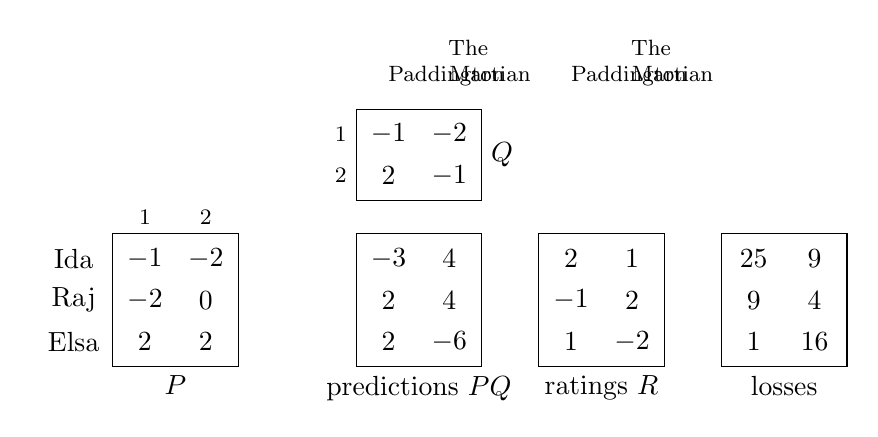
\begin{tikzpicture}
\matrix (m) [matrix of nodes, nodes in empty cells, row sep=1.5pt, column sep=3pt,
  nodes={minimum height=1.35em, minimum width=1.9em, anchor=center, inner sep=1pt}, column 1/.style={anchor=east}] {
 &  &  &  &  & |[text width=\headwidth, align=center, anchor=south, minimum height=0pt, font=\footnotesize]| Paddington\strut & |[text width=\headwidth, align=center, anchor=south, minimum height=0pt, font=\footnotesize]| The Martian\strut &  & |[text width=\headwidth, align=center, anchor=south, minimum height=0pt, font=\footnotesize]| Paddington\strut & |[text width=\headwidth, align=center, anchor=south, minimum height=0pt, font=\footnotesize]| The Martian\strut &  &  &  \\
 &  &  &  &  & $-1$ & $-2$ &  &  &  &  &  &  \\
 &  &  &  &  & $2$ & $-1$ &  &  &  &  &  &  \\
 & |[font=\footnotesize]| 1 & |[font=\footnotesize]| 2 &  &  &  &  &  &  &  &  &  &  \\
|[inner xsep=4pt]| Ida & $-1$ & $-2$ &  &  & $-3$ & $4$ &  & $2$ & $1$ &  & $25$ & $9$ \\
|[inner xsep=4pt]| Raj & $-2$ & $0$ &  &  & $2$ & $4$ &  & $-1$ & $2$ &  & $9$ & $4$ \\
|[inner xsep=4pt]| Elsa & $2$ & $2$ &  &  & $2$ & $-6$ &  & $1$ & $-2$ &  & $1$ & $16$ \\
};
\node[draw, inner sep=2pt, fit=(m-2-6)(m-3-7)] (Q) {};
\node[draw, inner sep=2pt, fit=(m-5-2)(m-7-3)] (P) {};
\node[draw, inner sep=2pt, fit=(m-5-6)(m-7-7)] (PQ) {};
\node[draw, inner sep=2pt, fit=(m-5-9)(m-7-10)] (R) {};
\node[draw, inner sep=2pt, fit=(m-5-12)(m-7-13)] (L) {};
\node[anchor=east, inner sep=3pt, font=\footnotesize] at (Q.west |- m-2-6) {1};
\node[anchor=east, inner sep=3pt, font=\footnotesize] at (Q.west |- m-3-6) {2};
\node[anchor=west, inner sep=3pt] at (Q.east) {$Q$};
\node[anchor=north, inner sep=3pt] at (P.south) {$P$};
\node[anchor=north, inner sep=3pt] at (PQ.south) {predictions $PQ$};
\node[anchor=north, inner sep=3pt] at (R.south) {ratings $R$};
\node[anchor=north, inner sep=3pt] at (L.south) {losses};
\end{tikzpicture}

\end{center}
Total loss: $25 + 9 + 9 + 4 + 1 + 16 = 64$.

\subsection{One number at a time}

For one number $w$ of $P$ or $Q$:
\begin{enumerate}
\item Before: the total loss.
\item After: the total loss with $w$ changed to $w + 0.01$.
\item Slope: $\nabla = (\text{after} - \text{before})/0.01$.
\item Update: $w \leftarrow w - \alpha \nabla$, with the step size $\alpha = 0.02$.
\end{enumerate}
A negative slope moves $w$ up, a positive slope moves it down. A round updates every number once, the numbers of
$P$ first. Rounds repeat until the total loss is below $0.001$.

Example: The Martian's second number, $w = -1$. Before: $64.00$. After, with $w = -0.99$: $63.72$. Slope:
$\nabla = -0.28/0.01 = -28$. Update: $w \leftarrow -1 - 0.02 \times (-28) = -0.44$; the total loss falls to
$50.86$. After $77$ rounds the total loss is below $0.001$ and every prediction is within $0.03$ of its rating.

Game: \PartTwo. Notebook: \NotebookMF, part 2.

\subsection{Gradient descent}

\term{Slope rule.} For a number $w$ and a known rating whose prediction contains $w$:
$2 \times \text{partner} \times (\text{prediction} - \text{rating})$, where the partner is the number that $w$
multiplies in that prediction. A rating whose prediction does not contain $w$ gives $0$.

\term{Slope of the total loss.} The sum of the slope rule over the known ratings. The slope measured with a change
of $0.01$ is close to it.

\term{Gradient.} The slopes of all numbers of $P$ and $Q$.

\term{Gradient descent.} Every number moves at once, $w \leftarrow w - \alpha \times \text{slope}$, again and again
until the total loss stops falling.

Example: from the first guess above, with $\alpha = 0.02$, one step takes the total loss from $64$ to $19.68$, and
$118$ steps take it below $0.0001$.

Game: \Optional. Notebook: \NotebookOpt, parts 3 and 4.

\subsection{Predicting unknown ratings}

The total loss uses the known ratings only. After the descent, $PQ$ has an entry for every customer and every
film; for an unknown rating, that entry is the prediction.

Example: real ratings from MovieLens\footnote{MovieLens ml-latest-small, GroupLens Research, University of
Minnesota. F.~Maxwell Harper and Joseph A.~Konstan, The MovieLens Datasets: History and Context, ACM Transactions on
Interactive Intelligent Systems 5(4), 2015.}, $10$ users and $12$ films, each rating the number of stars minus 3,
three ratings hidden. Gradient descent with $k = 2$, $\alpha = 3/117$ and $200$ steps takes the total loss of the
$117$ known ratings from $215.17$ to $29.35$. The hidden ratings and their predictions:
\begin{center}
% GENERATED by tools/notes_numbers.py: do not edit, run the script.
\begin{tabular}{|l|c|c|c|}
\hline
Film & MovieLens user & Prediction & Rating \\ \hline
Independence Day & 64 & $0.67$ & $0$ \\ \hline
Braveheart & 28 & $0.62$ & $0.5$ \\ \hline
Seven & 239 & $1.98$ & $2$ \\ \hline
\end{tabular}

\end{center}

Game: \PartThree.

\section{Games and notebooks}

Games, on the course site:

{\small
\begin{tabular}{@{}l@{\hspace{1.2em}}l@{}}
Once Upon a Video Store & {\footnotesize\url{https://eth-ainit-hs26.github.io/AINIT-PAGE/viz/we2/video-store/}} \\
Matchmaker, part one & {\footnotesize\url{https://eth-ainit-hs26.github.io/AINIT-PAGE/viz/we2/matchmaker-part-1/}} \\
Matchmaker, part two & {\footnotesize\url{https://eth-ainit-hs26.github.io/AINIT-PAGE/viz/we2/matchmaker-part-2/}} \\
Matchmaker, part three & {\footnotesize\url{https://eth-ainit-hs26.github.io/AINIT-PAGE/viz/we2/matchmaker-part-3/}} \\
Matchmaker, optional part & {\footnotesize\url{https://eth-ainit-hs26.github.io/AINIT-PAGE/viz/we2/matchmaker-optional/}} \\
\end{tabular}\par}

Notebooks, in the public repository \url{https://github.com/eth-ainit-hs26/w2-cx-public}. Each link opens a
notebook in Colab:

{\small
\begin{tabular}{@{}l@{\hspace{1.2em}}l@{}}
Nearest neighbors & \href{https://colab.research.google.com/github/eth-ainit-hs26/w2-cx-public/blob/main/01_cx_nearest_neighbours_student.ipynb}{student}, \href{https://colab.research.google.com/github/eth-ainit-hs26/w2-cx-public/blob/main/01_cx_nearest_neighbours_solutions.ipynb}{solutions} \\
Matrix factorization, parts 1 and 2 & \href{https://colab.research.google.com/github/eth-ainit-hs26/w2-cx-public/blob/main/02_cx_matrix_factorization_student.ipynb}{student}, \href{https://colab.research.google.com/github/eth-ainit-hs26/w2-cx-public/blob/main/02_cx_matrix_factorization_solutions.ipynb}{solutions} \\
Matrix factorization, optional parts 3 and 4 & \href{https://colab.research.google.com/github/eth-ainit-hs26/w2-cx-public/blob/main/02_cx_matrix_factorization_optional_student.ipynb}{student}, \href{https://colab.research.google.com/github/eth-ainit-hs26/w2-cx-public/blob/main/02_cx_matrix_factorization_optional_solutions.ipynb}{solutions} \\
\end{tabular}\par}

\end{document}
